\Chapter{Tervezés}

Itt kezdődik a dolgozat lényegi része, úgy értve, hogy a saját munka bemutatása.
Jellemzően ebben szerepelni szoktak blokkdiagramok, a program struktúrájával foglalkozó leírások.
Ehhez célszerű UML ábrákat (például osztály- és szekvenciadiagramokat) használni.

Amennyiben a dolgozat inkább kutatás jellegű, úgy itt lehet konkretizálni a kutatási módszertant, a kutatás tervezett lépéseit, az indoklást, hogy mit, miért és miért pont úgy érdemes csinálni, ahogyan az a későbbiekben majd részletezésre kerül.

Ebben a fejezetben az implementáció nem kell, hogy túl nagy szerepet kapjon.
Ez még csak a tervezési fázis.
(Nyilván ha olyan a téma, hogy magának az implementációnak a módjával foglalkozik, adott formális nyelvet mutat be, úgy a kódpéldákat már innen sem lehet kihagyni.)

\Section{Táblázatok}

Táblázatokhoz a \texttt{table} környezetet ajánlott használni.
Erre egy minta \aref{tab:minta}. táblázat.
A hivatkozáshoz az egyedi \texttt{label} értéke konvenció szerint \texttt{tab:} prefixszel kezdődik.

\begin{table}[h]
\centering
\caption{Minta táblázat. A táblázat felirata a táblázat felett kell legyen!}
\label{tab:minta}
\begin{tabular}{l|c|c|}
a & b & c \\
\hline
1 & 2 & 3 \\
4 & 5 & 6 \\
\hline
\end{tabular}
\end{table}

\Section{Ábrák}

Ábrákat a \texttt{figure} környezettel lehet használni.
A használatára egy példa \aref{fig:cimer}. ábrán látható.
Az \texttt{includegraphics} parancsba 
Az ábrák felirata az ábra alatt kell legyen.
Az ábrák hivatkozásához használt nevet konvenció szerint \texttt{fig:}-el célszerű kezdeni.

\begin{figure}[h]
\centering

\includegraphics[scale=0.3]{images/me_logo.png}
\caption{A Miskolci Egyetem címere.}
\label{fig:cimer}
\end{figure}

\Section{További környezetek}

A matematikai témájú dolgozatokban szükség lehet tételek és bizonyításaik megadására.
Ehhez szintén vannak készen elérhető környezetek.

\begin{definition}
Ez egy definíció
\end{definition}

\begin{lemma}
Ez egy lemma
\end{lemma}

\begin{theorem}
Ez egy tétel
\end{theorem}

\begin{proof}
Ez egy bizonyítás
\end{proof}

\begin{corollary}
Ez egy tétel
\end{corollary}

\begin{remark}
Ez egy megjegyzés
\end{remark}

\begin{example}
Ez egy példa
\end{example}

\section{Az alkalmazás működésének terve}

A cél egy olyan webalkalmazás létrehozása, amely lehetővé teszi XML-sémák feltöltését, az azok alapján dinamikusan előállított űrlapok kitöltését, valamint a kitöltött űrlap alapján XML-formátumba történő beküldése. A rendszer tervezése során fontos szempont, hogy az űrlapok létrehozását és kitöltését külön folyamatként lehessen kezelni. Ennek megfelelően a regisztrált felhasználók által létrehozott űrlapok egy egyedi hivatkozáson keresztül más személyek számára is elérhetővé válhatnak, így azok kitöltéséhez nem kell megadniuk a sémát.

Az alkalmazás használatához a felhasználóknak saját fiókot kell regisztrálni, majd bejelentkezni. A regisztrált felhasználók egy XML-séma feltöltésével készíthetnek egy dinamikus űrlapot. A feltöltött séma feldolgozása során a rendszernek fel kell ismernie az egyes elemek típusát, kötelezőségi feltételeit és egyéb megkötéseit, majd ezek alapján kell kialakítania a megfelelő beviteli mezőket és azok validációs szabályait.

A létrehozott űrlap elérését egy hivatkozás biztosítja majd. A séma tulajdonosa ezt a hivatkozást megoszthatja másokkal, akik így közvetlenül megnyithatják a kitöltőfelületet. Ennek köszönhetően az űrlap kitöltéséhez nem lesz szükség a projektkezelő felület használatára. A kitöltő számára az alkalmazásnak a séma alapján előállított űrlapot kell megjelenítenie, biztosítva az adatok megfelelő formátumú bevitelét és ellenőrzését.

Az űrlap beviteli elemei közé a továbbiak tartoznak:
\begin{itemize}
\item egysoros szöveg,
\item jelszómező,
\item email cím,
\item jelölőnégyzet,
\item rádiógomb,
\item szám mező,
\item dátum naptár,
\item többsoros szöveg,
\item legördülő lista,
\item csúszka.
\end{itemize}
A beviteli mező típusát a program automatikusan határozza meg, de lehetőség lesz, hogy a sémán belül további adatokat adjon meg a felhasználó, amivel a megadhatja a beviteli mezőt.

Az űrlap beküldése előtt a rendszernek ellenőriznie kell a megadott értékeket a feltöltött XML-sémában meghatározott feltételek alapján. Amennyiben az adatok megfelelnek az előírásoknak, az alkalmazásnak elő kell állítania a megfelelő szerkezetű XML-dokumentumot, majd azt továbbítja, hogy a szerveren letárolja. Hibás vagy hiányos adatok esetén a felhasználónak visszajelzést kell kapnia a javítandó mezőkről.

A beküldött dokumentumokat a séma tulajdonosa, majd külön felületen érheti el. Ezen az oldalon lesz lehetősége letölteni, vagy szükség esetén törölnie a beérkezett XML-dokumentumokat.


\begin{figure}[h]
\centering
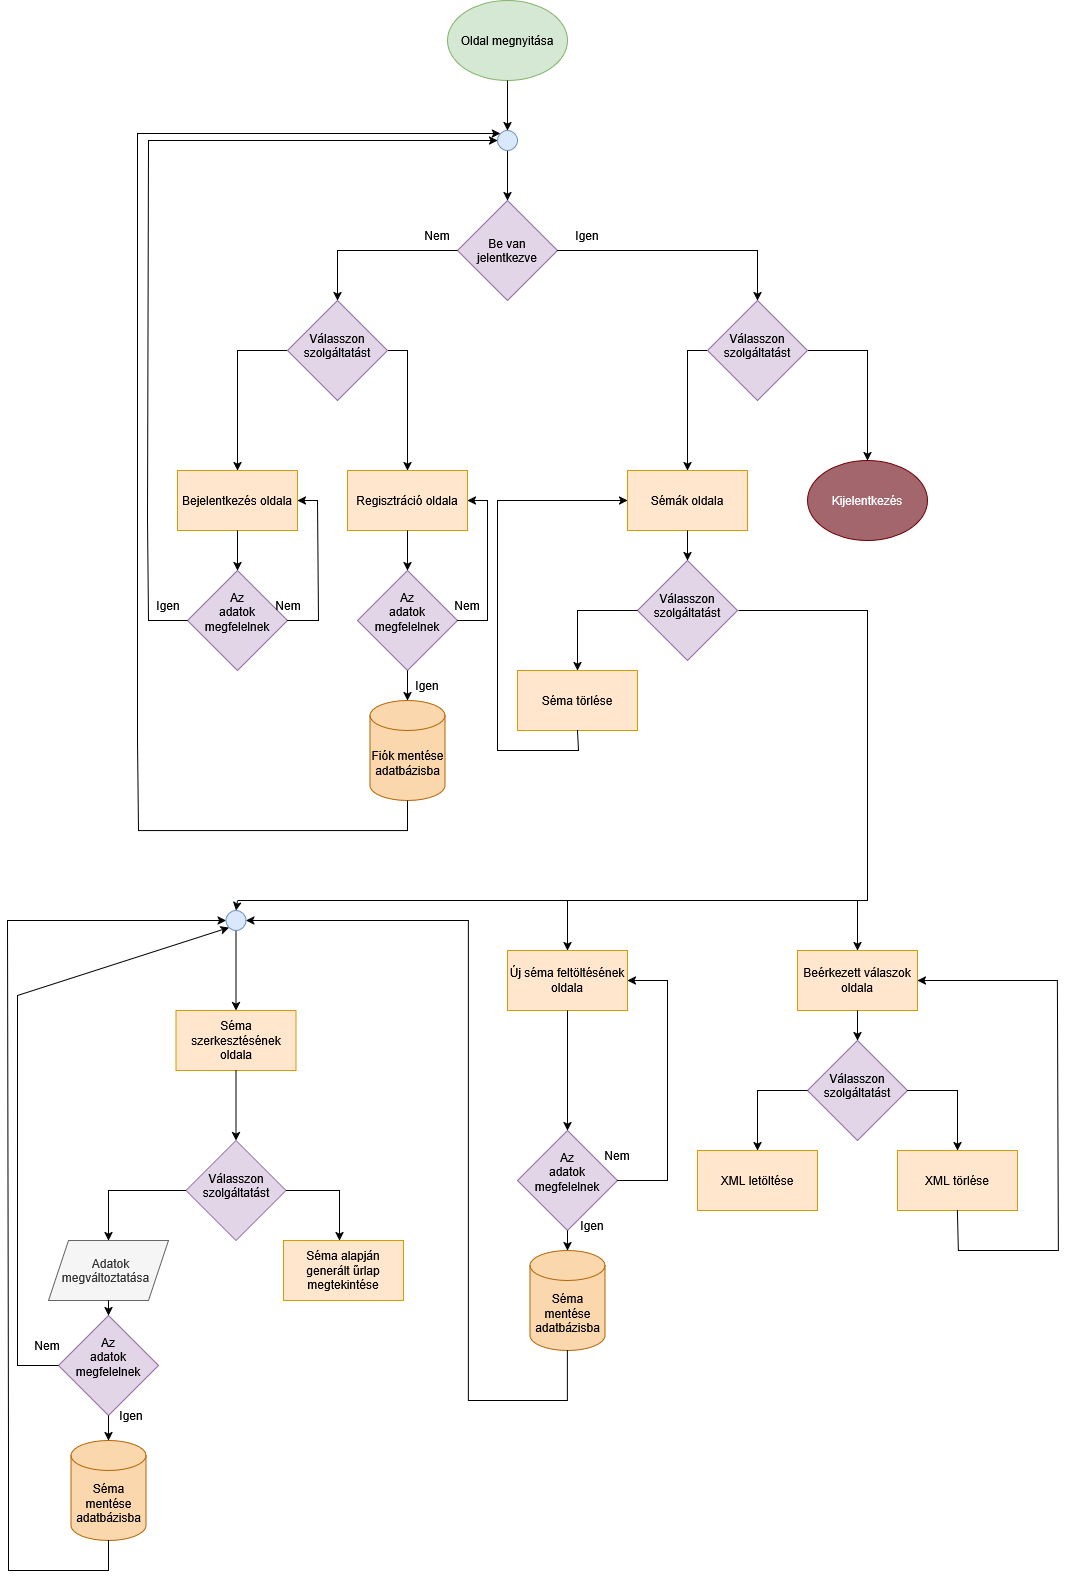
\includegraphics[width=\textwidth]{images/folyamatdiagram.png}
\caption{Az alkalmazás használatot ábrázoló folyamatdiagram.}
\label{fig:folyamat}
\end{figure}